\section{Adapted interfaces}


Since our application aims to help autistic people, the interface and the display of information are an important part of our project. Uncertainty and service disruptions are sources of anxiety for autistic people when using public transport \cite{2020ExperiencesYoungAutistic}, information must hence be brought to the user in a clear format and with no room for doubt.


Previous research revealed that autistic people and their caregivers rely a lot on images to share and receive information \cite{2018MobilityPoliciesExtraSmall}. Taking this into account, we decided to use pictograms to label areas that may prove to be stressful. At each step of the journey, the starting point of a given segment is represented by a dedicated icon. If the following steps contain segments where the user could be troubled by lights, sounds, or crowds, an orange icon is displayed, warning the user of the issues they may face. When taping on the icon, along with the usual step information, warning messages are displayed. Those messages specify what could be the issues on the segment.


\begin{figure}[H]
    \centering
    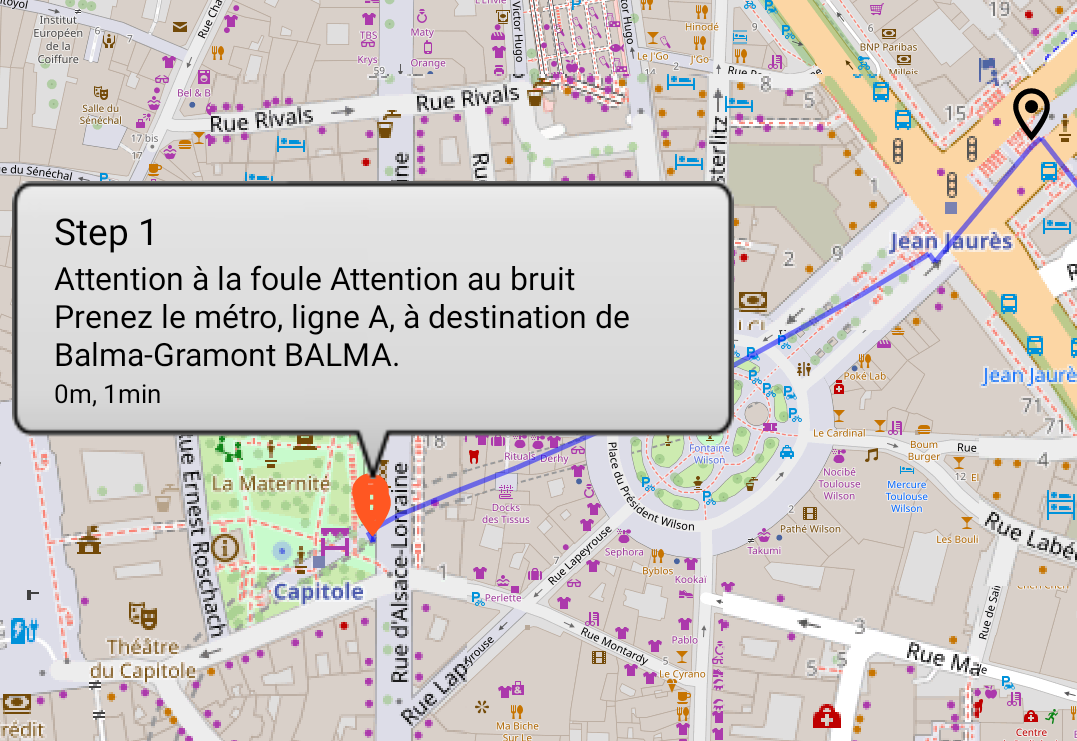
\includegraphics[scale=0.3]{img/step warning.png}
    \caption{Visualisation of a warning step}
    \label{fig:WarningStep}
\end{figure}


Finally, we conceived the journey planner as simply as possible, to only give necessary information to the user as to not overwhelm them and to remove any uncertainty. The Tisseo API usually returns different possible paths to travel between destinations, but our application chooses the best out of all the available options and returns only one path to the user. The Tisseo API also allows our app to line up with public transport schedules, and this information can be relayed to the user so that they know how long they will stay at one location.
